\documentclass[11pt]{beamer}
\usetheme{Madrid}
\usepackage[utf8]{inputenc}

\usepackage{hyperref}
\usepackage{amsmath}
\usepackage{amsfonts}
\usepackage{amssymb}
\usepackage{graphicx}
\DeclareMathOperator{\argmin}{argmin}
\usepackage{algorithmic}
\usepackage{algorithm}
\usepackage{wrapfig}
\usepackage{subcaption}
\graphicspath{{.}}

\usepackage{amsthm}
\theoremstyle{definition}
\newtheorem{exmp}{Example}[section]
\newtheorem{prop}{Proposition}[section]

\author{Hongda Li}
\title[TV Min and Nesterov Acc]{A Discussion on The Nesterov Momentum and Variants of FISTA with TV Minmizations Application}
% Informe o seu email de contato no comando a seguir
% Por exemplo, alcebiades.col@ufes.br
\newcommand{\email}{lalala@lala.la}
\setbeamercovered{transparent}
\setbeamertemplate{navigation symbols}{}
%\logo{}
\institute[]{UBC Okangan}
\date{\today}
\subject{Subject Title }

% ---------------------------------------------------------
% Selecione um estilo de referência
\bibliographystyle{IEEEtran}

%\bibliographystyle{abbrv}
%\setbeamertemplate{bibliography item}{\insertbiblabel}
% ---------------------------------------------------------

% ---------------------------------------------------------
\newtheorem{remark}{Remark}
\newtheorem{assumption}{Assumption}




\begin{document}

\begin{frame}
    \titlepage
\end{frame}

\begin{frame}{Presentation Overview}
    \tableofcontents
\end{frame}

\section{Paper Under Review}
    \begin{frame}{Paper Under Review}
        \begin{center}
            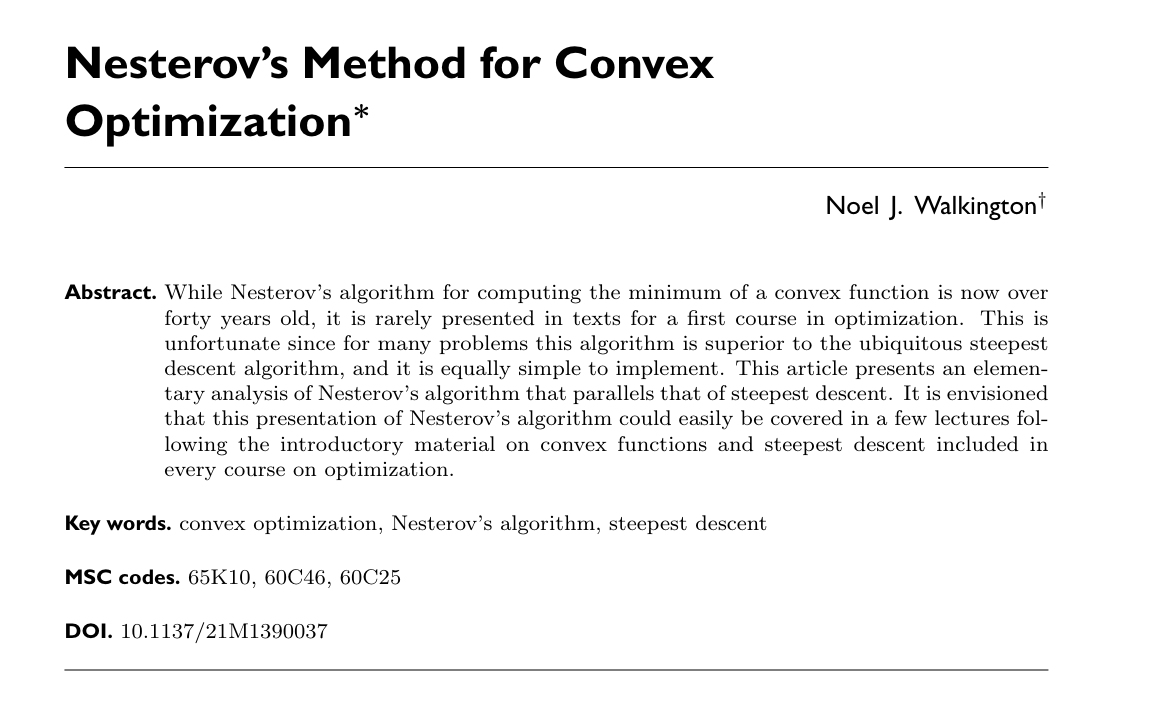
\includegraphics[width=10cm]{Assets/paper-titlepage.png}    
        \end{center}
        Noel J. Walkington, SIAM REVIEW Jun 2023 Education, Volume 65 Number 2, pp. 539-562. \cite{noel_nesterovs_nodate}
    \end{frame}
    
    % \begin{frame}{Presentation Outline and Objective}
    %     \begin{itemize}
    %         \item [1.] Introducing the Application of TV Minimization for Signal Recovery.
    %         \item [2.] Literature Review. 
    %         \item [3.] Nesterov lower bound complexity claim clarified. 
    %         \item [4.] Our proof for V-FISTA convergence under strong convexity inspired by Beck \cite[10.7.7]{beck_first-order_nodate}. 
    %         \item [5.] Some exciting numerical results for our method, which we refer to as ``The method of Spectral Momentum''. 
    %     \end{itemize}
    % \end{frame}

\section{TV Minimizations}
    \begin{frame}{Formulation of Total Variational Minimization}
        Total Variance minimization (TV) problem recovers the digital signal from observations of a signal with noise. 
        Let $u(t):[0, 1]\mapsto \mathbb R$ be the signal and $\hat u$ be a noisy observation, then
        \begin{block}{Variational Formulation}
            \[
                f(u) = \int_0^1 \frac{1}{2} 
                (u(t) - \hat u(t))^2 + \alpha |u'(t)|dt. 
            \]    
        \end{block}
        \begin{itemize}
            \item \textcolor{red}{Minimizing $f(u)$ with pentalty term constant $\alpha > 0$ yield a recovered signal. }
            \item Penalization helps recover an original signal $u$ that is assumed to be piecewise constant with bounded variation. 
        \end{itemize}
    \end{frame}
    \begin{frame}{Formulation of Total Variational Minimization}
        \begin{block}{Variational Formulation}
            \[
                f(u) = \int_0^1 \frac{1}{2} 
                (u(t) - \hat u(t))^2 + \alpha |u'(t)|dt. 
            \]    
        \end{block}
        Solving the problem on modern computing platforms requires discretization of the problem. 
        Here is a list of helpful quantities for discretized formulation. 
        \begin{itemize}
            \item Let $u = [u_0\; \cdots \; u_{N}]^T \in $, be a vector. 
            This is the variable we optimize to get a solution. 
            \item Let $t_0< \cdots<  t_i <\cdots <t_N$ be a sequence of time for each observed value: $u_i$. 
            \item Let $h_i=t_{i} - t_{i - 1}$ be the elapse of time between $u_i, u_{i - 1}$, for all $i \ge 1$. 
            \item Let $C\in \mathbb R^{N\times (N + 1)}$ be a bi-diagonal matrix with $-1/h_{i}, 1/h_{i + 1}, i = 1,\cdots, N$ on the diagonal and the super diagonal. 
            This is a finite difference matrix. 
            \item Let $D= \text{diag}(h_1/2, h_1,\cdots, h_N, h_{N}/2) \in \mathbb R^{(N + 1)\times(N + 1)}$. 
        \end{itemize}
    \end{frame}

    \begin{frame}{Discretized Model}
        The following would be the discretized model formulation. \footnote{See our report for the omitted details.}
        Recall $D$ is diagonal, strictly positive entry, $C\in \mathbb R^{N\times N+ 1}$ is bidiagonal. 
        \begin{block}{Discretized Formulation}
            \[ 
                f(u) = \frac{1}{2}\langle u - \hat u, D(u - \hat u)\rangle + \alpha \Vert Cu\Vert_1.     
            \]
        \end{block}
        If we were to use the Forward-Backward(FB) splitting, then we have unresolved implementation difficulties: 
        \pause
        \begin{itemize}
            \item [1.] ADMM, Chambolle Pock, would apply; 
                \textcolor{red}{however, when using the FB Splitting, $\alpha\Vert Cu\Vert_1$ would be prox unfriendly. }
            \item [2.] Prox over $\alpha \Vert C u\Vert_1$ is possible with $D$ being bi-diagonal, but it would be a hassle if done for generic $C$. 
            \textcolor{red}{Hence, we reformulate and use the Lagrangian dual. }
        \end{itemize}
    \end{frame}

    \begin{frame}{Dual}
        \begin{block}{The Dual Reformulation}
            \begin{align*}
                - g(\lambda) = -\frac{1}{2}    \Vert C^T\lambda\Vert^2_{D^{-1}} - 
                \langle \hat u, C^T \lambda\rangle - 
                \delta_{[-\alpha, \alpha]^N}(\lambda). 
            \end{align*}
            See my report for omitted details.    
        \end{block}
        \begin{itemize}
            \item Fact: $u = \hat u + D^{-1}C^T\lambda$, for the primal. 
            \item $D^{-1}$ is Positive Definite and diagonal, very easy to invert. 
            \item $g(\lambda)$ would be strongly convex. 
        \end{itemize}
    \end{frame}

    \begin{frame}{Numerical Results}
        We implemented in Julia \cite{bezanson_julia_2017}, with several variants of FISTA, producing 
        \begin{figure}[H]
            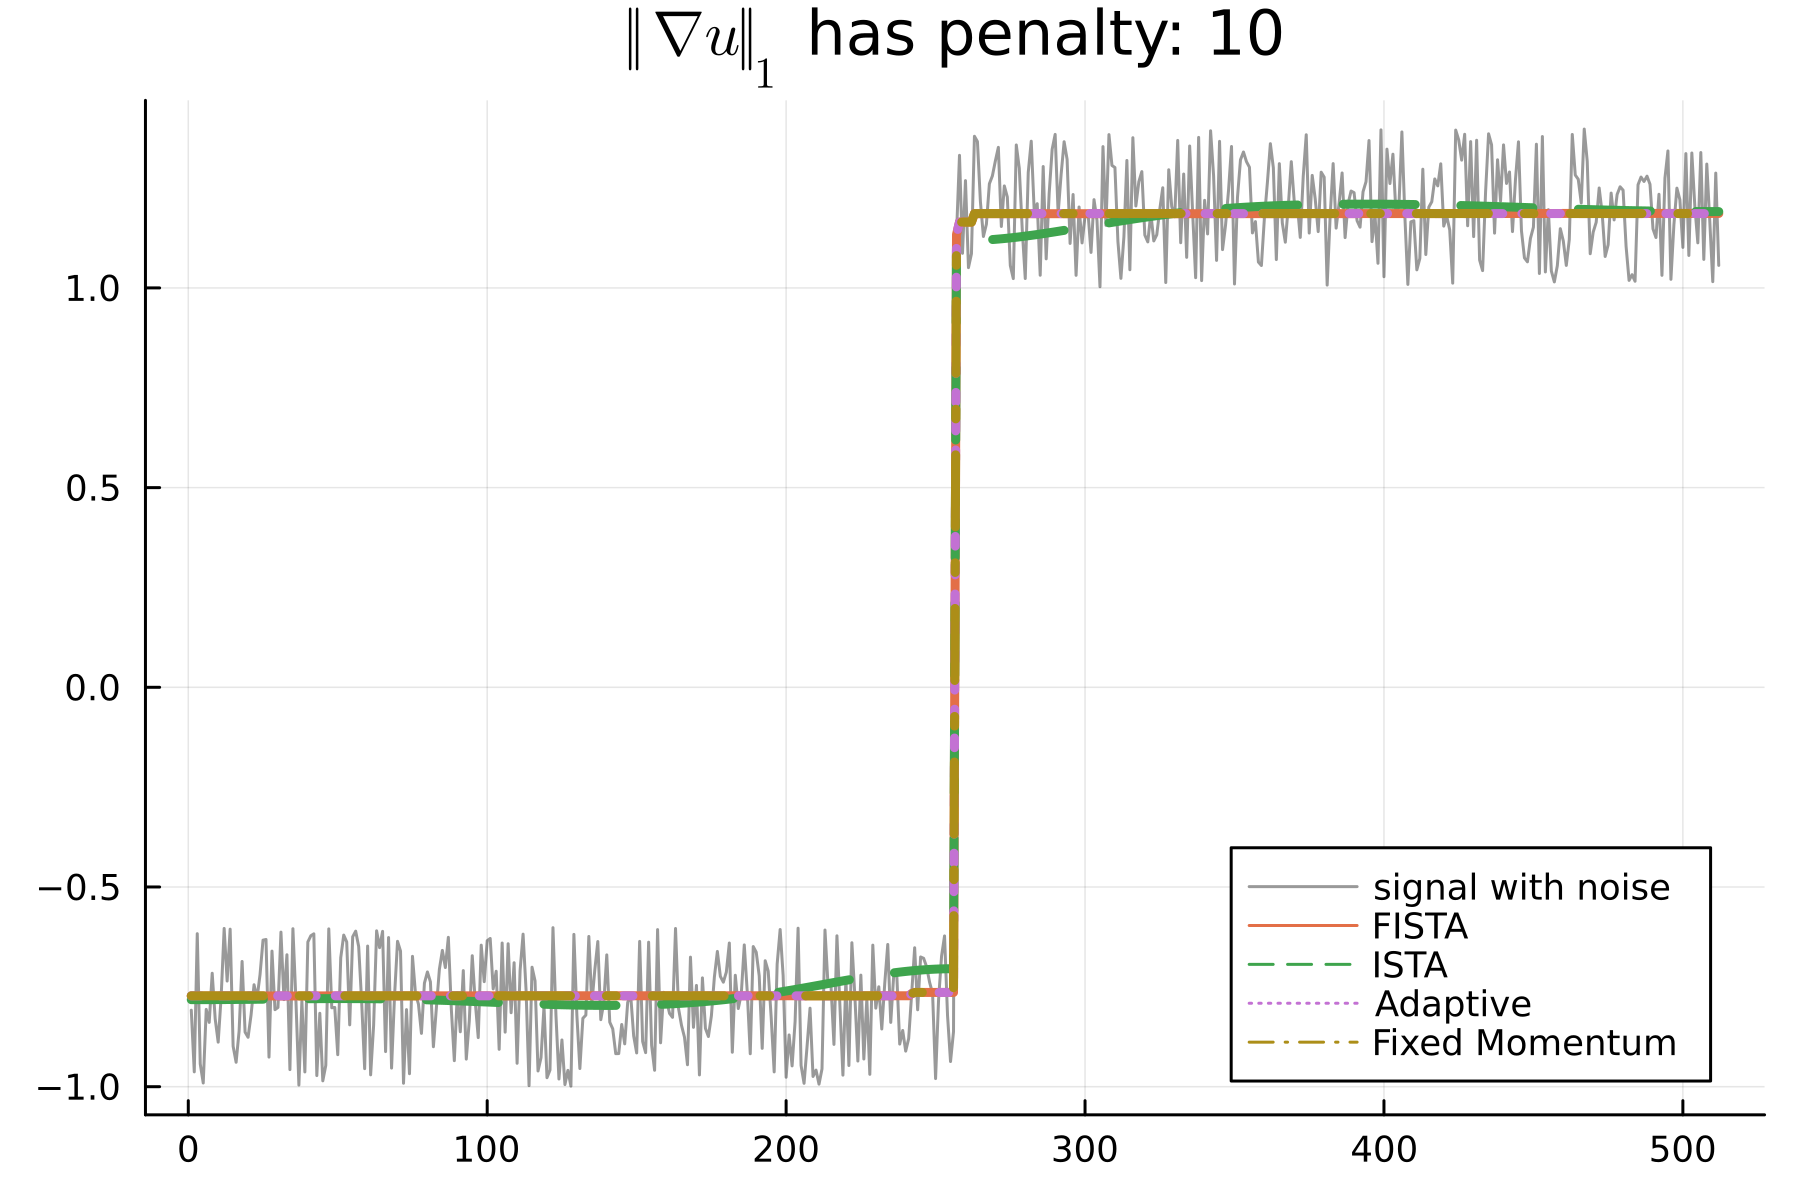
\includegraphics[width=9cm]{Assets/recovered_signal.png}    
        \end{figure}
        {\small
            See GitHub repository \href{https://github.com/iluvjava/Proximal-Gradient/tree/main/applications}{\textcolor{cyan}{here}} for our code implementation. 
            See our report for more numerical experiments. 
        }
    \end{frame}

    \begin{frame}{Convergence Results}
        \begin{figure}
            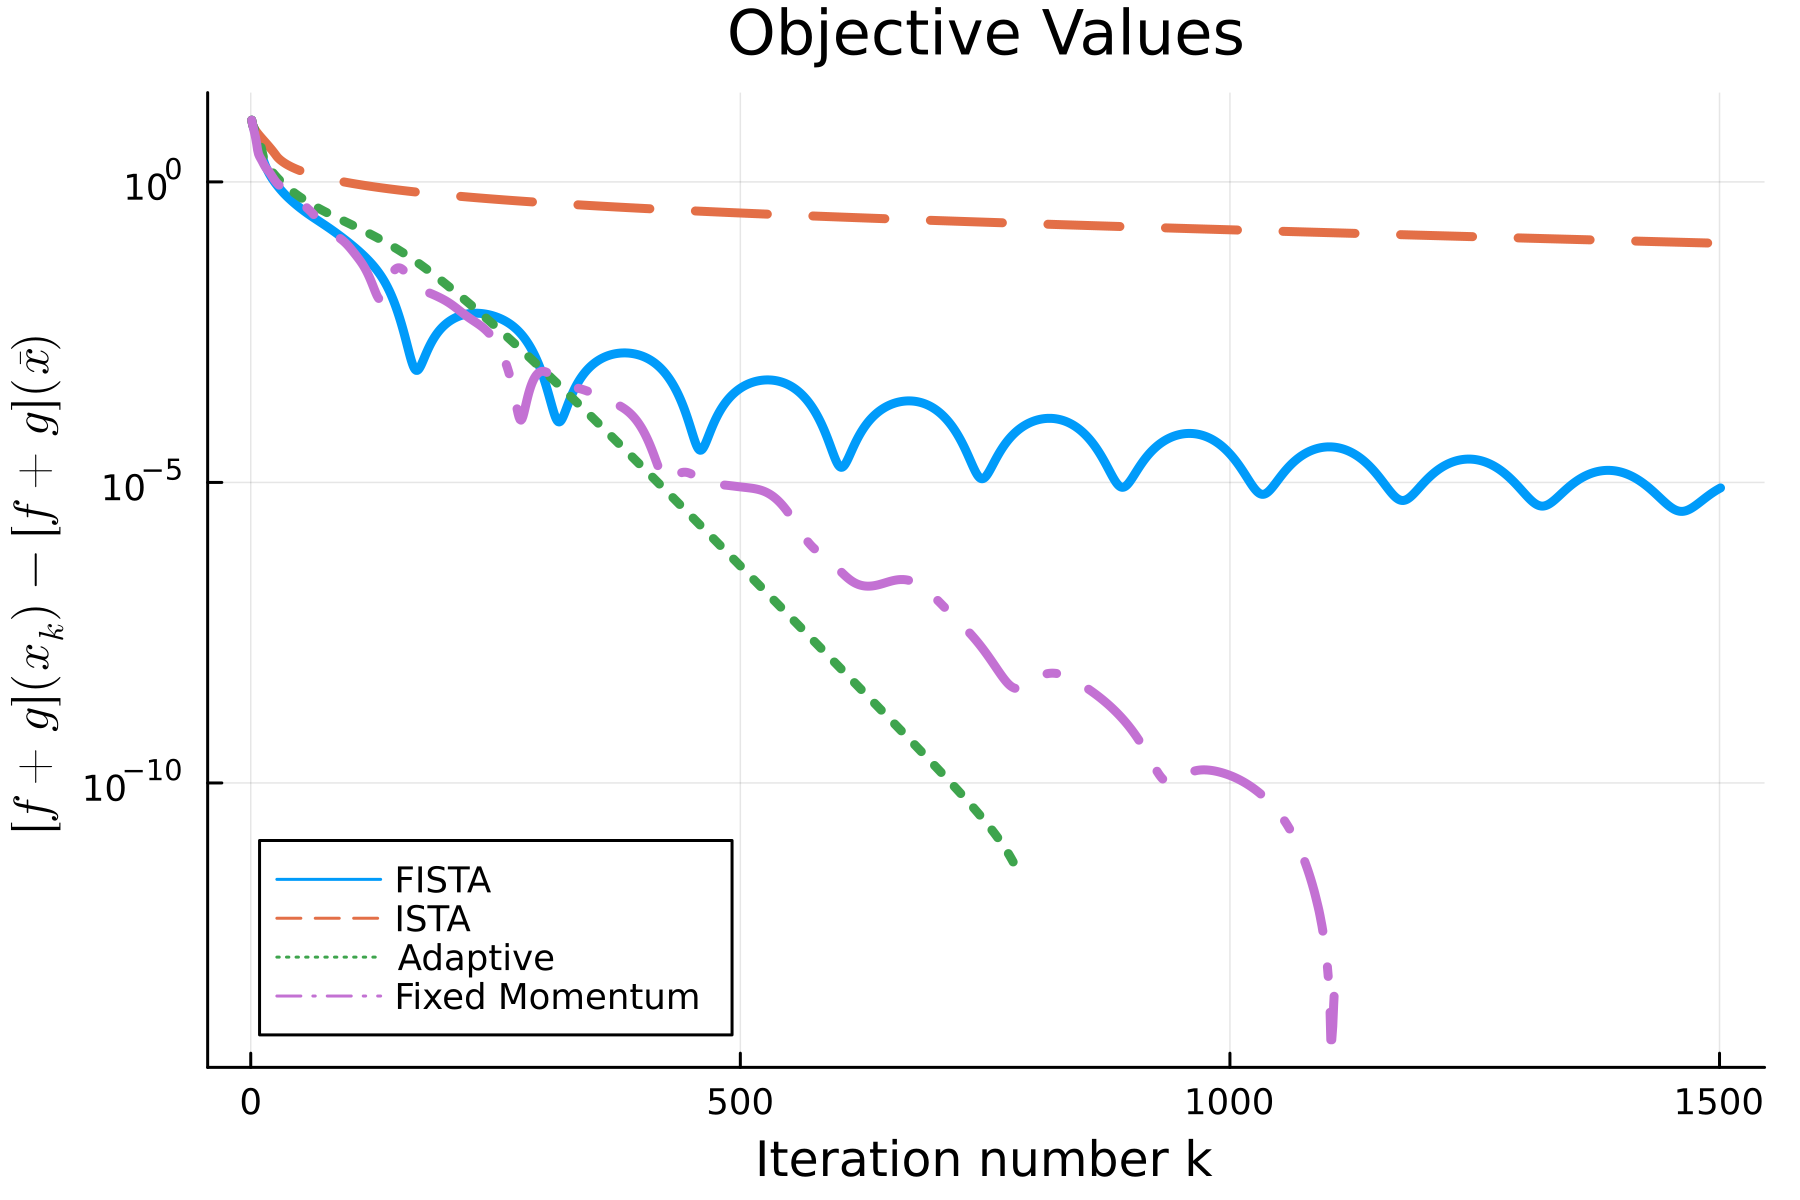
\includegraphics[width=10cm]{Assets/obj_vals.png}
        \end{figure}
    \end{frame}

    \begin{frame}{One Big Bummer}
        \begin{figure}
            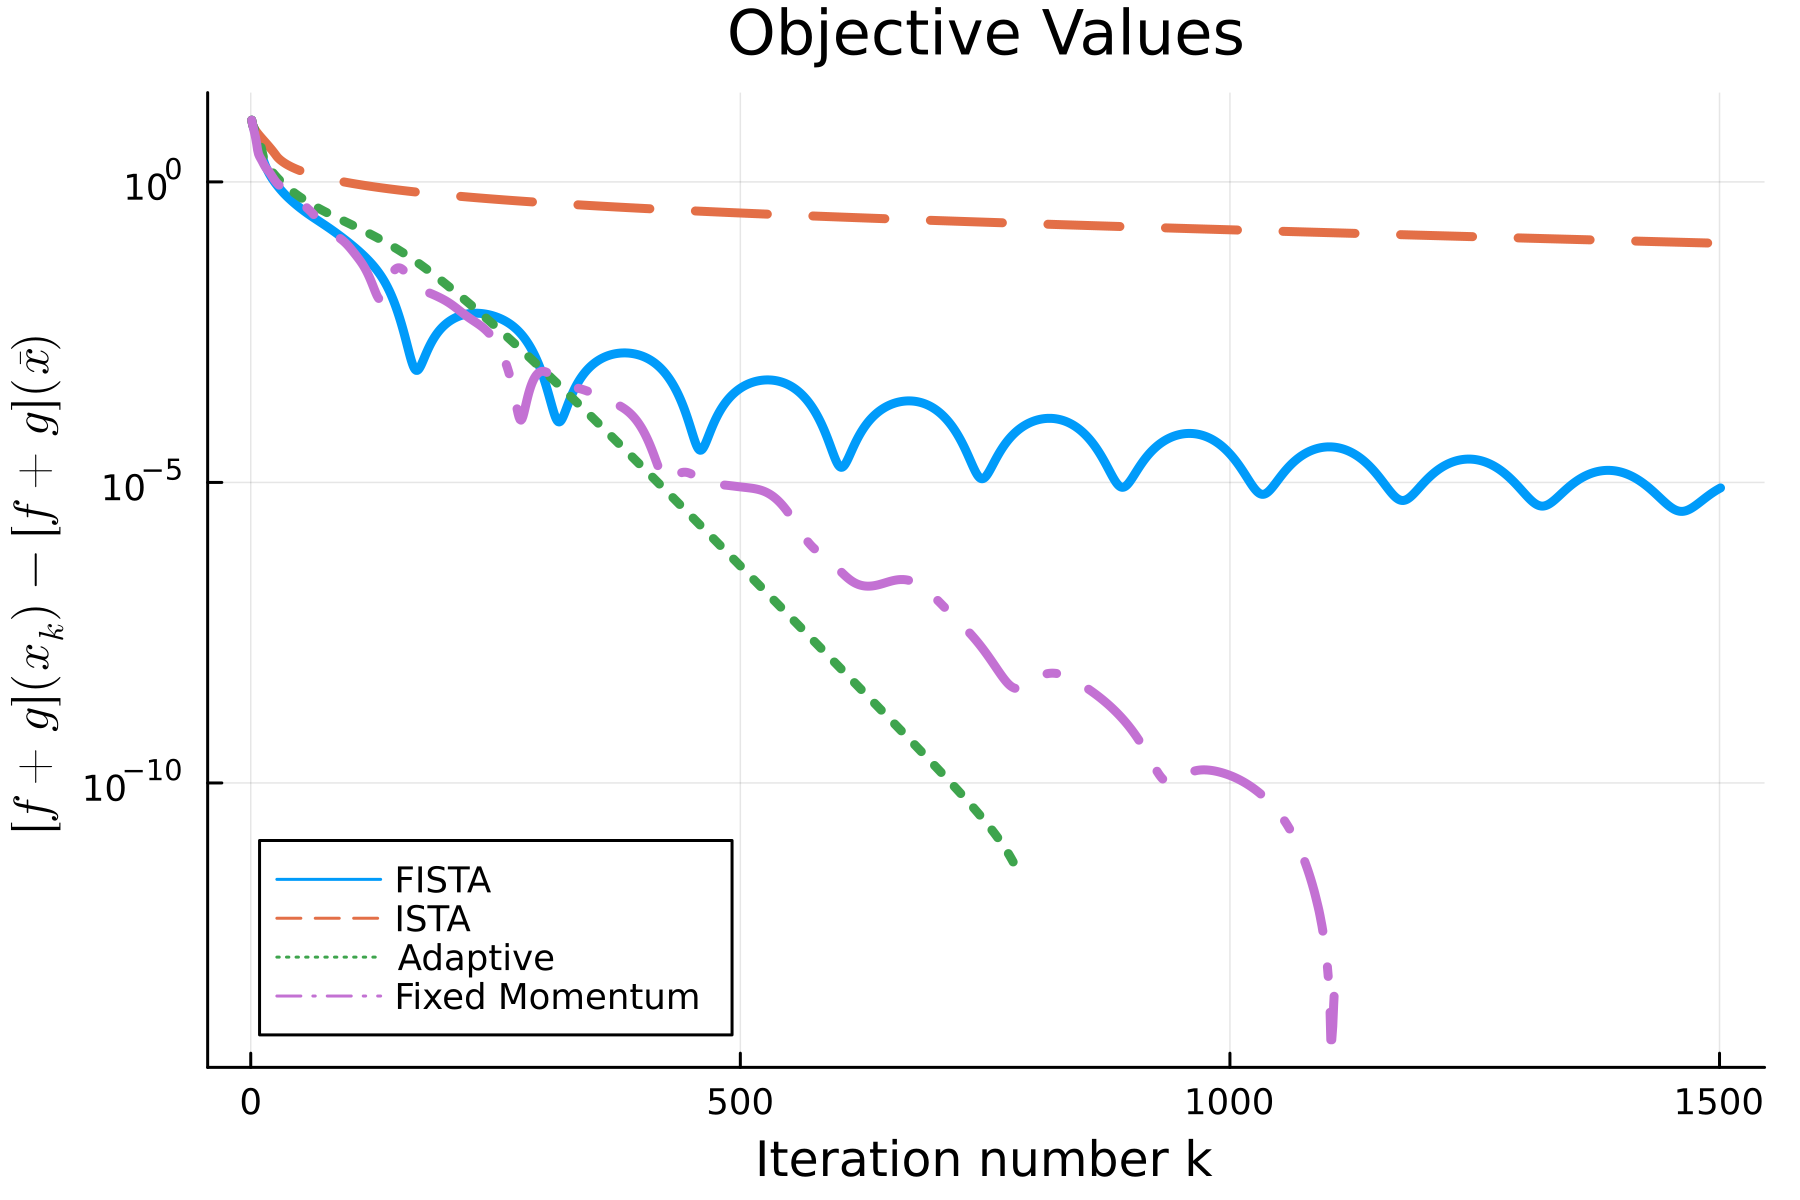
\includegraphics[width=6cm]{Assets/obj_vals.png}
        \end{figure}
        Main observations
        \begin{itemize}
            \item [1.] FISTA is \textcolor{red}{non-robust to strong convexity}; the above suggests that it experiences the same $\mathcal O (1/k^2)$. 
            \item [2.] However, ISTA would be $\mathcal O((1 - 1/\kappa)^k)$ under strong convexity, with $\kappa = L/\sigma$, for $L$-Lipschitz smooth and $\sigma$ strongly on the smooth part of the FB splitting objective. 
        \end{itemize}
    \end{frame}
        
\section{Literature Review}
    \begin{frame}{Generic FISTA}
        We introduce algorithm \ref*{alg:generic_FISTA} to expedite presentation. Consider Smooth, non-smooth additive composite objective $F = g + h$. 
        \begin{block}{A Good Template}
            \begin{algorithm}[H]
                \begin{algorithmic}[1]
                    \STATE{\textbf{Input: }($g, h, x^{(0)}$)}
                    \STATE{$y^{(0)} = x^{(0)}$, $\kappa = L/\sigma$} 
                    \FOR{$k = 0, 1, \cdots$}
                        \STATE{$x^{(k + 1)} = T_L y^{(k)}; T_L(x) = \text{prox}_{L^{-1}h}(x - L^{-1}\nabla g(x))$}
                        \STATE{$y^{(k + 1)} = x^{(k + 1)} + \theta_{k + 1}(x^{(k + 1)} - x^{(k)})$}
                        \STATE{Execute subroutine $\mathcal S$. }
                    \ENDFOR
                \end{algorithmic}
                \caption{Generic FISTA}
                \label{alg:generic_FISTA}
            \end{algorithm}
        \end{block}
        Changing $T_L$, $\theta_{k + 1}$, and $\mathcal S$ yield different variants. 
    \end{frame}

    \begin{frame}{Variant (1.), FISTA Original}
        \begin{algorithm}[H]
            \begin{tiny}
                \begin{algorithmic}[1]
                    \STATE{\textbf{Input: }($g, h, x^{(0)}$)}
                    \STATE{$y^{(0)} = x^{(0)}$, $\kappa = L/\sigma$} 
                    \FOR{$k = 0, 1, \cdots$}
                        \STATE{$x^{(k + 1)} = T_L y^{(k)}$}
                        \STATE{$y^{(k + 1)} = x^{(k + 1)} + \theta_{k + 1}(x^{(k + 1)} - x^{(k)})$}
                        \STATE{Execute subroutine $\mathcal S$. }
                    \ENDFOR
                \end{algorithmic}
                \caption{Generic FISTA}    
            \end{tiny}
        \end{algorithm}
        Original FISTA proposed by Beck \cite{beck_fast_2009-1} has 
        \begin{itemize}
            \item $\theta_{k + 1} = (t_k - 1)/t_{k + 1}$, $t_{k + 1}(t_{k + 1} - 1) = t_{k}^2$, $t_0 = 1$. 
            \item It achieves $\mathcal O(1/k^2)$ on the objective value; it doesn't improve for strongly convex function $g$. 
            \item No known proof for the convergence of the iterates. 
            \item $T_L(x) = \text{prox}_{L^{-1}h}(x - L^{-1}\nabla g(x))$. 
        \end{itemize}
    \end{frame}

    \begin{frame}{Variant (2.), Chambolle, Dossal (Skippable)}
        \begin{algorithm}[H]
            \begin{tiny}
                \begin{algorithmic}[1]
                    \STATE{\textbf{Input: }($g, h, x^{(0)}$)}
                    \STATE{$y^{(0)} = x^{(0)}$, $\kappa = L/\sigma$} 
                    \FOR{$k = 0, 1, \cdots$}
                        \STATE{$x^{(k + 1)} = T_L y^{(k)}$}
                        \STATE{$y^{(k + 1)} = x^{(k + 1)} + \theta_{k + 1}(x^{(k + 1)} - x^{(k)})$}
                        \STATE{Execute subroutine $\mathcal S$. }
                    \ENDFOR
                \end{algorithmic}
                \caption{Generic FISTA}    
            \end{tiny}
        \end{algorithm}
        From Chambolle, Dossal \cite{chambolle_convergence_2015}, 
        \begin{itemize}
            \item $t_{k + 1} = (n + a - 1)/a, \theta_{k + 1} = (t_{k} - 1)/t_{k + 1}$, for $a > 2$. 
            \item Proved in Chambolle, Dossal \cite[thm 4.1]{chambolle_convergence_2015}, its iterates of this version of FISTA exhibit convergence. 
            \item $T_L$ is the same as (1.); it experiences the same convergence rate for the function objective. 
        \end{itemize}
    \end{frame}

    \begin{frame}{Variant (3.) (Also known as V-FISTA), From Beck}
        \begin{algorithm}[H]
            \begin{tiny}
                \begin{algorithmic}[1]
                    \STATE{\textbf{Input: }($g, h, x^{(0)}$)}
                    \STATE{$y^{(0)} = x^{(0)}$, $\kappa = L/\sigma$} 
                    \FOR{$k = 0, 1, \cdots$}
                        \STATE{$x^{(k + 1)} = T_L y^{(k)}$}
                        \STATE{$y^{(k + 1)} = x^{(k + 1)} + \theta_{k + 1}(x^{(k + 1)} - x^{(k)})$}
                        \STATE{Execute subroutine $\mathcal S$. }
                    \ENDFOR
                \end{algorithmic}
                \caption{Generic FISTA}    
            \end{tiny}
        \end{algorithm}
        Proposed in Beck \cite{beck_first-order_nodate}, and also Nesterov \cite{nesterov_lecture_2018}. 
        \begin{itemize}
            \item has $\theta_{k + 1} = (\sqrt{\kappa} - 1)/(\sqrt{\kappa} + 1)$. 
            \item Only for $g$ with strong convexity (Or the weaker condition such as Quadratic Growth). 
            \item Has $\mathcal O((1 - 1/\textcolor{red}{\sqrt{\kappa}})^k)$, for both objective value and iterates. 
        \end{itemize}
    \end{frame}

    \begin{frame}{Spectral Momentum Variants (4.)}
        V-FISTA is simple but requires knowledge of $\sigma$, the strong convexity index; it is a troublemaker. 
        \begin{itemize}
            \item Exact estimation would involve inverting the Hessian or a closed-form formula tailored for a specific problem. 
            \item Over estimation of $\sigma$ invalidates the linear convergence results. 
            \item Under estimation of $\sigma$ slows down the linear-convergence. 
        \end{itemize}
        \textcolor{red}{To overcome this, we propose a real-time overestimation of $\sigma$ using}
        \[
            \sigma \le \langle \nabla g(y^{(k + 1)}) - \nabla g(y^{(k)}), y^{(k + 1)} - y^{(k)}\rangle/ 
                    \Vert y^{(k + 1)} - y^{(k)}\Vert^2. 
        \]
        We call this \textbf{Spectral Momentum}. 
        The same formula is used for spectral stepsizes \cite[4.1]{goldstein_field_2016}, also known as (Barzilai-Borwein method) when applied to gradient descent. 
        However, we used it on the momentum term. 
        Its efficacy was demonstrated at the start of the talk. 
        We are not sure why it works so well. 
    \end{frame}

    \begin{frame}{MFISTA Variants (5.)}
        \begin{algorithm}[H]
            \begin{tiny}
                \begin{algorithmic}[1]
                    \STATE{\textbf{Input: }($g, h, x^{(0)}$)}
                    \STATE{$y^{(0)} = x^{(0)}$, $\kappa = L/\sigma$} 
                    \FOR{$k = 0, 1, \cdots$}
                        \STATE{$x^{(k + 1)} = T_L y^{(k)}$}
                        \STATE{$y^{(k + 1)} = x^{(k + 1)} + \theta_{k + 1}(x^{(k + 1)} - x^{(k)})$}
                        \STATE{Execute subroutine $\mathcal S$. }
                    \ENDFOR
                \end{algorithmic}
                \caption{Generic FISTA}    
            \end{tiny}
        \end{algorithm}
        MFISTA in Beck \cite{beck_fast_2009} is produced by adding $\mathcal S$ to be the procedure
        \[
            (y^{(k + 1)}, t_{k + 1}) = \begin{cases}
                (x^{(k + 1)}, 1) & F(y^{(k + 1)}) > F(x^{(k + 1)}),
                \\
                (y^{(k + 1)}, t_{k + 1}) & \text{else}. 
            \end{cases}
        \]
        Recall 
        $\theta_{k + 1} = (t_k - 1)/t_{k + 1}$, $t_{k + 1}(t_{k + 1} - 1) = t_{k}^2$, $t_0 = 1$. 
    \end{frame}

    \begin{frame}{MFISTA Drawbacks (Skippable)}
        MFISTA was an early attempt at improving FISTA. 
        \begin{itemize}
            \item [1.] Requires frequent computing of the objective, slowing it by a constant factor compared to FISTA. 
            \item [2.] There is no better convergence rate than $\mathcal O(1/k^2)$ from our research. 
        \end{itemize}
    \end{frame}

    \begin{frame}{FISTA Restart Refuses to Die}
        However, the idea of restarting FISTA refuses to go away. 
        \\
        \begin{itemize}
            \item Asymptotic linear convergence of conditional restart by Alamo et al. \cite{alamo_restart_2019},\cite{alamo_gradient_2019} et al., and Fercoq \cite{fercoq_adaptive_2019}, under strong convexity, or local quadratic growth. 
            \item Parameter Free FISTA with automatic restart by Aujol et al. \cite{aujol_parameter-free_2023}, linear convergence $\mathcal O(\exp(-K\sqrt{\kappa}n))$ ($n$ is the iteration counter) on quadratic growth with proofs, no parameters needed.
        \end{itemize}
    \end{frame}

    \begin{frame}{Theories of Nesterov Momentum}
        Frontier developments of theories for Nesterov Momentum are not dying either. 
        \begin{itemize}
            \item [1.] Su et al. \cite{su_differential_2015} identified a second-order ODE that is the exact limit of the variant (1.). 
            \item [2.] In Attouch and Peypouquet \cite{attouch_rate_2016}, they showed a $o(1/k^2)$ convergence rate of variant (2.) based on the ODE understanding. 
            \item [3.] In Nesterov \cite{nesterov_lecture_2018}, he proposed a generic algorithm that can derive variants (1.), (3.), and more. 
            \item [4.] In Ahn and Sra \cite{ahn_understanding_2022}
            they derived a lot of variants of APGs using the Proximal Point method of Rockafellar and discussed the unified theme of a ``similar triangle." 
        \end{itemize}
    \end{frame}

    \begin{frame}{The Most Recent and Hardcore Developement}
        The paper is titled ``Computer-Assisted Design of Accelerated Composite Optimization Methods: OptISTA" by Jang et al. \cite{jang_computer-assisted_2023}.
        They updated the manuscript On Nov 1st, 2023. 
        \begin{itemize}
            % \item Based on the Performance Estimation Problem, they phrase the search of the fastest possible first-order algorithm(more on this later) as a QCQP. 
            % \item They squeeze out a constant factor on the convergence of the original FISTA. 
            \item They also proved a lower bound for their OptISTA, showing its exact optimality. 
            \item They claim they had concluded the search for the fastest first-order method. 
        \end{itemize}
        That leads to the question: ``Why do we call Nesterov's acceleration method optimal?" 
        What is optimality for an algorithm? 
    \end{frame}
    % \begin{frame}{Moral of the Story}
    %     This is the general trajectory: 
    %     \begin{itemize}
    %         \item Improve the algorithm's robustness and applications.  
    %         \item Weaken the conditions and add more convergence proofs for a broader scope. 
    %         \item Searching for a general framework of understanding for the class of the Nesterov acceleration method. 
    %         \item Connects with various other ideas to improve theoretical understanding.
    %         \item Extremely hardcore algorithmic tricks and improvements to squeeze out that last bit of performance. 
    %     \end{itemize}
    %     Working on FISTA would amount to competing against some of the brightest researchers. 
    % \end{frame}
    
   

\section{Nesterov Lower Bound}
\newcommand*{\GAfirst}{\text{GA}^{\text{1st}}}
    \begin{frame}{First-Order Methods}
        What we can do is to understand at least Nesterov's claim on lower complexity bound and why we believe there is a mistake in Walkington \cite[theorem 2.4]{noel_nesterovs_nodate}. 
        \begin{definition}[First Order Method]
            We are in $\mathbb R^n$ for now. Given $x^{(0)} \in \mathbb R^n$, an iterative algorithm generates sequence of $\left(x^{(n)}\right)_{n \in \mathbb N}$ in the space. All $\mathcal A \in \GAfirst$ satisfy that 
            \begin{align*}
                 x^{(j + 1)}:= \mathcal A_f^{j + 1}x^{(0)} \in \left\{x^{(0)}\right\} + 
                \text{span}\left\{\nabla f\left(x^{(i)}\right)\right\}_{i = 1}^{j} \quad \forall f, \forall 1\le j \le k -1. 
            \end{align*}
        \end{definition}
        We adapted the above definition from Nesterov \cite[2.1.4]{nesterov_lecture_2018}. 
        We came up with two examples for the definition. 
    \end{frame}  
    \begin{frame}{Fixed-Step Descent}
        \begin{exmp}[Fixed Step Descent]
            The method of fixed-step gradient descent, $x^{(k + 1)} = x^{(k)} - L^{-1}\nabla f(x^{(k)})$ is $ \bar {\mathcal A}\in \GAfirst$ achieves a maximal decrease in objective value \textcolor{red}{for all $f\in \mathcal F_{L}^{1, 1}$} for some $x^{(k)}\in \mathbb R^n$, it can be understood as 
            \[
                \bar {\mathcal A} \in 
                \underset{_{\mathcal A\in \GAfirst}}{\text{argmin}}
                \max_{f\in \mathcal F_L^{1, 1}} \left\lbrace
                    f\left(
                        \mathcal A_f x^{(k)}
                    \right)
                \right\rbrace. \textcolor{gray}{\quad\triangleright\; \text{Only a single iteration.}}
            \]
        \end{exmp}
        \begin{exmp}[Steepest Descent]
            \textcolor{red}{Fix some $f, x^{(k)}$}, the method of steepest descent would be $\bar {\mathcal A}\in \GAfirst$ and it's 
            \[
                \bar {\mathcal A}\in  \underset{\mathcal A \in \GAfirst}{\text{argmin}}
                \left\lbrace
                    f\left(
                        \mathcal A_f x^{(k)}
                    \right)
                \right\rbrace. 
            \]
        \end{exmp}
    \end{frame}
    
    \begin{frame}{Nesterov Lower Complexity Bound}
        The following is Nesterov \cite[Thm 2.1.7]{nesterov_lecture_2018}. 
        \begin{theorem}[Nesterov's Claim of Lower Bound]\label{thm:nesterov_lower_bnd}
            \textcolor{red}{For any $1\le k \le (n - 1)/2$, for all $x^{(0)}\in \mathbb R^n$, there exists a Lipschitz smooth convex function in $\mathbb R^n$} such that for all algorithm from $\GAfirst$, we have the lower bound for the optimality gap for the function values and its iterates: 
            \[
                f\left(x^{(k)}\right) - f^* \ge 
                \frac{3L \Vert x - x^*\Vert^2}{32(k + 1)^2}, 
                \quad \Vert x^{(k)} - x^*\Vert^2 \ge \frac{1}{8} \Vert x^{(0)} - x^*\Vert^2.     
            \]
            Where $x^*$ is the minimizer of $f$, so that $f(x^*) = \inf_{x}f(x)$. 
        \end{theorem}
        We emphasize that it didn't fix the function $f$, but it fixes the iteration counter $k$. 
        
    \end{frame}
    \begin{frame}{Walkington's claim of Lower Bound}
        We now quote Walkington \cite[theorem 2.4]{noel_nesterovs_nodate}
        \begin{theorem}[Walkington's Claim of Lower Bound]
            Let $X$ be an infinite-dimensional Hilbert Space and set $x^{(0)} =\mathbf 0$. \textcolor{red}{There exists a convex function $f: X\mapsto \mathbb R$ with Lipschitz gradient and minimum $f(x_*) > -\infty$ such that for any} sequence satisfying 
            \begin{align*}
                x_{i + 1}\in \text{Span}\left\lbrace
                    \nabla f(x^{(0)}), \nabla f(x^{(1)}), \cdots, \nabla f(x^{(i)})
                \right\rbrace, 
                \quad i = 0, 1, 2, \cdots, 
            \end{align*}
            there holds 
            \begin{align*}
                \min_{1\le i \le n}
                f(x_i) - f(x_*) \ge 
                \frac{3L\Vert x_1 - x_*\Vert^2}{32(n + 1)^2}, 
            \end{align*}
            where $L$ is the Lipschitz constant of the gradient. 
        \end{theorem}\label{thm:walkington_lowerbound}
    \end{frame}
    \begin{frame}{The Differences Between Their Claims}
        \begin{itemize}
            \item Walkingon claimed there exists a single function from $\mathcal F_{L}^{1,1}(\mathcal H)$ that introduces the lower bound for all values of $k$, and all algorithms from $\GAfirst$, but the latter didn't claim that. 
            \item The difference would remain in infinite dimension Hilbert space if we generalize Nesterov's lower bound claim. 
            \item No contradiction from Attouch and Peypouquet \cite{attouch_rate_2016} on $o(1/k^2)$ because they fixed $\Phi$ in the proof. 
        \end{itemize}
        There is no proof after Walkington's claim; we can't know if he had his way of proving the latter claim. 
        It makes us think it is likely a missed detail in his writing. 
    \end{frame}

 

\section{V-FISTA Under Strong Convexity}

    \begin{frame}{Preparing for Strong Convexity Convergence of V-FISTA}
        To understand the proof, we introduce the following quantities for simplicity. 
        \begin{itemize}
            \item [1.] $s^{(k)} = x^{(k)} - x^{(k - 1)}$, the velocity vector,
            for all $k\ge 1$. 
            \item [2.] $e^{(k)} = x^{(k)} - \bar x$, the error vector at the kth iteration, for $k \ge 0$. 
            \item [3.] $\theta_k = (t_k -1)/(t_k + 1)$, which is the momentum step size. 
            \item [4.] $u^{(k)} = \bar x + t_{k}(x^{(k - 1)} - x^{(k)}) - x^{(k - 1)}$, the error term extrapolated with the velocity. We take $u^{(0)} = \bar x - x^{(0)}$. 
            \item [5.] $\delta_k = f(x^{(k)}) - f_{\text{opt}}$, with $f_{\text{opt}} = f(\bar x) = \inf_x f(x)$. 
            \item [6.] The quantity $R_k$ plays a crucial role in the proof; it's
            {\small
                $$
                R_k = 
                \frac{\sigma(t_{k + 1} - 1)}{2}
                \left\Vert
                    x^{(k)} - \bar x
                \right\Vert^2 
                - 
                \frac{L - \sigma}{2}
                \left\Vert
                    \bar x + t_{k + 1}\left( x^{(k)} - y^{(k)}\right) - x^{(k)}
                \right\Vert^2
                $$
            }
            \item [7.] $\kappa = L/\sigma$, the condition number, it would be that $\kappa \ge 0$. 
            \item [8.] $q = \sigma/L$, the reciprical of the condition number. It would be that $q \in (0, 1)$. 
        \end{itemize}

    \end{frame}

    \begin{frame}{V-FISTA Generic Convergence}
        \begin{lemma}[Generic Convergence Results]\label{lemma:convergence-prep}
            If there exists a sequence $(t_k)_{k\in \mathbb N}, C_k$ such that 
            \begin{align}
                \begin{cases}
                    \frac{C_k}{t_{k + 1}^2} = \frac{L(1 - t^{-1}_{k + 1})}{2t_{k}^2}
                    \\
                    R_k + C_k\left\Vert
                        u^{(k)}
                    \right\Vert^2 \ge 0, 
                \end{cases}
            \end{align}
            then 
            \begin{align*}
                \delta_{k + 1}
                \le 
                \left(
                    \prod_{i = 0}^{k} (1 - t_k^{-1})
                \right)\left(
                    \delta_0 + \frac{L}{2t_0^2}\left\Vert
                        u^{(0)}
                    \right\Vert^2
                \right). 
            \end{align*}
        \end{lemma}
        \begin{proof}
            In the appendix of the report. 
        \end{proof}
    \end{frame}
    \begin{frame}{A Sufficient Condition for Convergence}
        \begin{prop}[Sufficient Conditions for Generic Convergence]
            If the sequence $(t_k)_{k \ge \mathbb N}$ satisfies 
            \begin{itemize}
                \item [1.] $t_{k + 1} = 1 + \frac{t_k^2(1 - q)}{t_k + 1}$, 
                \item [2.] and $t_{k + 1} \ge t_k + 1 - t_k^2q$, 
                \item [3.] and $t_k > 1$ for all $k\ge 0$, 
            \end{itemize}
            make \hyperref[lemma:convergence-prep]{lemma \ref*{lemma:convergence-prep}} (Generic Convergence Results) true. 
        \end{prop}
        \begin{proof}
            In the appendix of the report. 
        \end{proof}
    \end{frame}

    \begin{frame}{Fixed Momentum Convergence}
        \begin{prop}
            The choice of $t_k = t_{k + 1} = \sqrt{\frac{L}{\sigma}}$ for all $k \ge 0$, then proposition (Sufficient Conditions for Generic Convergence) is true. 
            Hence, the V-FISTA variant (3.) has a convergence rate bound 
            \[
                \delta_{k + 1}
                \le 
                \left(
                    1 - \frac{1}{\sqrt{\kappa}}
                \right)^k\left(
                    \delta_0 + \frac{L}{2t_0^2}\left\Vert
                        u^{(0)}
                    \right\Vert^2
                \right).        
            \]
        \end{prop}
    \end{frame}
    \begin{frame}
        \begin{proof}
            we have 
            \begin{align*}
                \frac{t_{k + 1} - 1}{t^2_k(1 - q)}
                    -
                \frac{1}{t_k + 1} &= 0
                \quad 
                \triangleright\; \text{by } t_{k + 1} = t_k, \text{ then}
                \\
                \frac{t - 1}{t^2(1 - q)} &= \frac{1}{t + 1}
                \\
                t^2(1 - q) 
                &= t^2 - 1
                \\
                t^2q &= 1
                \\
                t &= \pm \sqrt{\frac{L}{\sigma}}, 
            \end{align*}
            with $t_k > 1$ it has to be $t_k = \sqrt{\frac{L}{\sigma}}$ for all $k \ge 0$. 
            With that we have $t_{k + 1} = t_{k} + 1 - t_k^2 q = t_k + 1 - 1 = t_k$, hence the inequality is also satisfied. 
        \end{proof}        
    \end{frame}


    
\section{References}
    \begin{frame}[allowframebreaks]{References}
        
        \bibliography{refs.bib}
    \end{frame}

\end{document}